\section{Technology Selection}
\subsection{Technology Stack}

\begin{figure}[H] 
    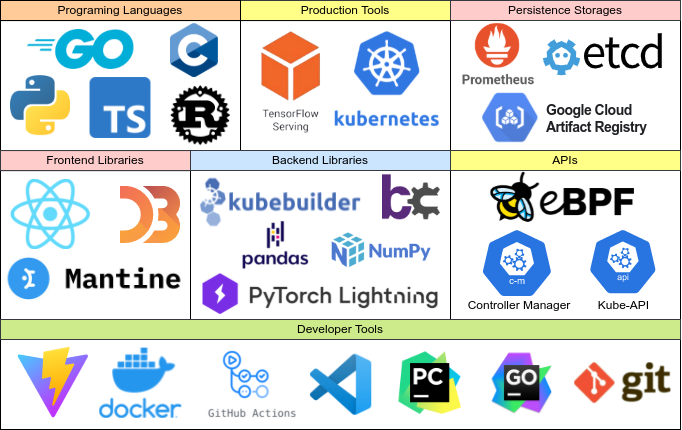
\includegraphics[width=13cm]{assets/implementation/technology-stack.png}
    \caption{Technology stack (self-composed)}
    \label{fig:technology-stack}
\end{figure}

At a grasp, this seems like a lot of toolings for a project of undergraduate level but each and every tool and technology listed here provide a vital functionality to make the final prototype efficient and reliable as much as possible in order to stand through to the design goals listed above.

\subsection{Programming Language}

This project was built using five different programming languages which were chosen due to their unique features that are required from different components in the system.

\begin{itemize}[noitemsep,nolistsep] 
    \item \textbf{GoLang} - Go is a programming language invented by Google that took a lot of inspiration from C but with modern features like memory safety, automatic garbage collection, and built-in concurrency. Due to this nature Go was used to build Kubernetes itself and almost all the tooling around Kubernetes relies on as their language of choice. Since this project tries to extend some functionality of Kubernetes, it was highly recommended to use Go to built parts of the system that interface with Kubernetes tooling.
    \item \textbf{Python} - Python is known as the go-to language for data science but in this project, Python had another critical role. There is a library called BCC which streamlines the connection to the Linux \ac{ebpf} API. So both data science and telemetry extraction components are built using Python.
    \item \textbf{C} - Linux \ac{ebpf} API allows userspace applications to submit some sandboxed programs into kernel space at runtime and the kernel responsible for compiling and executing them along with kernel calls. But since this is a Linux kernel feature all the sandboxed programs need to be written in C so the kernel can understand it.
    \item \textbf{TypeScript} - For frontend applications, programming languages are limited to Javascript and TypeScript. The TypeScript was chosen for this project since TypeScript offers a lot of compile-time checks which prevent accidental bugs from sneaking into the production application.
    \item \textbf{Rust} - Out of all tools and technologies this may be the only replaceable technology. Rust will be used in the \ac{sherlock} module to interface with the machine learning model. Even though Python or even Go could be viable alternatives to this, Rust has the lowest memory and CPU footprint of any modern programming language. Since one of the design goals of this project is to have the lowest overhead possible author was settled on relying on Rust for this task.
\end{itemize}



\subsection{Libraries Utilized}
Software libraries prevent software engineers from reinventing the wheel every time they want to perform some common functionality. This is done by empowering them with abstractions they can use to perform the task they wanted so they can focus on important things. To build this project a number of libraries were used both in UI and backend components.


\subsubsection{Frontend}
\begin{itemize}[noitemsep,nolistsep] 
    \item \textbf{ReactJS} - Since this is a hosted application a web-based UI made more sense. In order to build a web-based frontend, there are a few common methods, it is possible to use a vanilla HTML stack and build everything from scratch but for this project, UIs needs to be interactive and that left the author with three viable choices, ReactJS, VueJS, and Svelte. Since the author was more familiar with ReactJS he chose to rely on it for the UI implementation.
    \item \textbf{Mantine} - Mantine is a React component library which helps developers to use the prebuilt component like date pickers without having to code them from scratch. Viable alternatives for this is Boostrap, MaterialUI, and Ant Design. The author settled on Mantine due to its user-friendliness and rich TypeScript support.
    \item \textbf{Force Graph} - force-graph is a UI library that helps to create interactive graphs. This library was used to create the service topology graph. There weren't any alternatives for this that allowed to render directed graphs with interactivity.
\end{itemize}


\subsubsection{Backend}
\begin{itemize}[noitemsep,nolistsep] 
    \item \textbf{Kubebuilder} - Kubebuilder is a SDK that is used to build Custom Kubernetes Operators. This is created and maintained by the Kubernetes special interest group themself along with the community support. The only viable alternative for this is called Operator SDK which is developed by the community with the support of RedHat. Since the author had prior experience with Kubebuilder and its inner working, it was decided to rely upon it.
    \item \textbf{BCC} - BCC is a frontend to Linux \ac{ebpf} API which makes deploying kernel probes and retrieving data from them very easy. Other than relying on C interfaces this was the only viable solution. 
    \item \textbf{Pandas} - Pandas is a data manipulation and an analysis library that was used in both \ac{gazer} and \ac{sherlock} module.
    \item \textbf{Numpy} - Is considered a holy grail when it comes to data science work in Python. Even libraries like Tensorflow and PyTorch rely on this for manipulation of multi-dimensional arrays and matrices. In the training phase of \ac{sherlock}, NumPy was heavily used to preprocess the datasets.
    \item \textbf{Keras} - Keras is an abstraction on top of Tensorflow which help to create a deep learning model with minimum boilerplate code.
    
    %PyTorch Lightning is a layer of abstraction on top of the PyTorch library. The author chose to opt-into the PyTorch ecosystem rather than the Tensorflow ecosystem because, during the last 1-2 years Tensorflow got a lot of criticism to for being unoptimized for modern data science. The author also wanted some hands-on experience working with PyTorch since the industry seems to be moving towards PyTorch dominated era.
\end{itemize}

\subsection{Persistence Storages}

\begin{itemize}[noitemsep,nolistsep] 
    \item \textbf{Prometheus} - Prometheus is a time series database that doubles as a data scraping agent. Prometheus uses the pull method in contrast to normal pushing methods to update the database. During the requirement engineering phase, it was discovered the vast majority of companies rely on Prometheus. % So for this project author decided to rely on it as the primary database for storing metric data due to its popularity and well integration with Kubernetes.
    \item \textbf{etcd} - etcd is a key-value data store which is built into the core of Kubernetes. The \ac{lazy-koala-operator} relies on this to both sync up the monitoring config with \ac{gazer} instances as well as keep track of all the monitored services.
    \item \textbf{Github Container Registry} - This stores all the built containers, so that the Kubernetes cluster can easily pull down spin copies of them. Eventhough there are alternatives like DockerHub, Github Container Registry was used due to the tight integration with Github.  
    % Artifact Registry stores the trained models and docker containers. Viable alternatives for this are Github Container Registry, DockerHub, and Azure Container Registry. GCP Artifact Registry was chosen for this due to it's competitive pricing and cutting-edge features like AI-powered vulnerability scanning. 
\end{itemize}

\subsection{Developer Tools Utilized}
\begin{itemize}[noitemsep,nolistsep] 
    \item \textbf{Vite} - A Javascript build tool that can convert TypeScript code into well-optimized Javascript. Vite was selected over webpack due to its efficiency in build times.
    \item \textbf{Docker} - A container management tool, which can pack software into a lightweight self-containing package that can be deployed in Kubernetes.
    \item \textbf{Github Actions} - Automated CI/CD platform which is built into Github platform.
    \item \textbf{VSCode} - Code editor used to create frontend UIs.
    \item \textbf{PyCharm} - IDE used to develop \ac{gazer} and \ac{sherlock}.
    \item \textbf{GoLand} - IDE used to develop the \ac{lazy-koala-operator}.
    \item \textbf{Git} - Version control tool that was used to keep track of changes between releases.
\end{itemize}

\subsection{Production Tools}
\begin{itemize}[noitemsep,nolistsep] 
    \item \textbf{Tensorflow Servings} - Production grade machine learning model serving system written in C++ to be efficient as possible.
    \item \textbf{Kubernetes} - Host the entire system along with a distributed system that's get monitored.
\end{itemize}

\subsection{Summary of Technology Selection}

\begin{longtable}{|p{43mm}|p{110mm}|}
    \hline
    \textbf{Component} &
    \textbf{Tools/Technologies Used} \\ \hline

    \ac{lazy-koala-operator} &
    Go, etcd, Kubebuilder, Kube-API, Controller Manager, GoLand \\ \hline

    \ac{gazer} &
    C, Python, Prometheus, BCC, Pandas, \ac{ebpf}, Kube-API, PyCharm \\ \hline

    \ac{sherlock} - Training Phase &
    Python, Prometheus, Pandas, Numpy, Keras, PyCharm \\ \hline

    \ac{sherlock} - Production &
    Rust, Prometheus, TF-Servings, Github Container Registry\\ \hline

    User Interface &
    TypeScript, React, Mantine, D3.js, Vite, VSCode \\ \hline

    Common for all &
    Docker, Github Actions, Git, Kubernetes \\ \hline

    \caption{Summary of technology selection (self-composed)}
\end{longtable}